\vspace{-3cm}\chapter{题目2:创建自己的GUI图形}

\section{2.1 题目}

在阅读 TestDraw、DrawPanel 和 MyLine 类定义的基础上,为 MyCircle 和 MyRectangle 添加
相应的代码,以便让 TestDraw 程序可以绘制圆形和长方形。
\begin{enumerate}
	\item 创建上面提到的两个类型,包括必要的该类型的数据成员、构造方法(可以利用重载技术,
		使该类型具有多种构造能力)、以及必不可少的一个成员方法:
		\begin{lstlisting}[language = Java]
	public void draw(Graphics g)
		\end{lstlisting}
		上面成员方法中的参数 g 为类型 java.awt.Graphics,使用这个类来绘制所需要的图形,该类型的使用可以在 JDK API 中查找。注意:
		\begin{itemize}
			\item DrawPanel 的构造函数中提供了对 MyCircle 和 MyRectangle 类型数组的支持。
			\item 尽可能为 MyCircle 类和 MyRectangle 类提供多样的构造函数,体会重载以及理解构造函数的意义
			(构造函数之间通过 this 传递的方式也要多练)。
		\end{itemize}
	\item 不难注意到上面的代码复用率极低,大刀破斧的修改 DrawPanel 类的数据成员、构造函数等,使其具有可
		以接收绘制任何(包括已有的和未来的)具有相同行为的图形类型。为了达到代码复用的目的,可能修改的不止 DrawPanel 类。
\end{enumerate}
	
在实验报告中书写本题的设计环节部分时,请使用 UML 的类图进行阐述。

\section{2.2 题目分析}
本题分为两部分

\subsection{2.2.1 创建类}

\begin{itemize}
	\item \textbf{Field}. 参考几何学知识,用三个 int 变量计算圆心坐标( x\_position )和半径( y\_position )以确定 MyCircle 的位置,
	用两个 Color 类分别表示线颜色和填充颜色。MyRectangle 的位置则需要四个 int 变量表示左下角和右上角坐标(或者说x和y坐标的上界和下界)。
	\item \textbf{Constructor}. MyCircle 和 MyRectangle 类的构造函数编写过程和 MyTime 的过程类似,比较枯燥乏味,区别仅限于一个是自己构思,
	一个是参考测试代码,故在此略过,细节可以查看2.4的主干代码展示和附录的所有代码展示;
	\item \textbf{Other Method}. 这部分需要调用 Graphics 的方法来编写类的 draw 方法,一些细节值得注意:
	\begin{itemize}
		\item Panel 的坐标原点在左上方,这和一般的思路可能有差异;
		\item 查询 Graphics 的方法可知,绘制椭圆(圆形)的方法Oval是通过右上角点的坐标、短轴和长轴对圆定位的,这和现实生活的习惯不符;
	\end{itemize}
	\item \textbf{Test}. 对已有的TestDraw类修改可以使其测试 MyCircle 类和 MyRectangle 类
\end{itemize}

\subsection{2.2.2 提高代码复用性}
分析 DrawPanel 的代码,尤其是针对不同类的处理程序,并比较 MyLine, MyCircle 和 MyRectangle 三个类不难发现,有大量重复代码,所以可以设计
一个 MyShape 作为父类,考虑到一般不会出现未实例化的 MyShape,且每个 MyShape 的子类都会有自己对draw的方法实现,而
目前并未看到除此之外他们的关联,这里暂时把 MyShape 定义为抽象类。

这样就可以取消冗余而丑陋的利用 final int 和 case 作为选择,而转为直接对 MyShape 数组操作,以后新的图形类型只需 extends MyShape 即可。
除此之外当然也需要使已定义的图形类型继承 MyShape.

考虑到题目三的便利,这里再将 MyShape 的 draw 函数剥离出来,定义为 Drawable 接口,从而实现对任一实现了 Drawable 的类的绘制功能。

\section{2.3 结果展示}

\begin{figure}[H]
	\centering
	\begin{subfigure}{0.4\textwidth}
		\centering
		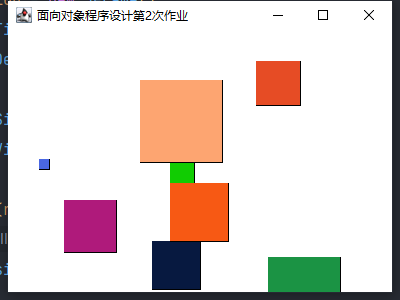
\includegraphics[width = 1\textwidth]{../pic/2/2.3.1.png}
		\caption{MyRectangle 测试绘制结果}
	\end{subfigure}
	\begin{subfigure}{0.4\linewidth}
		\centering
		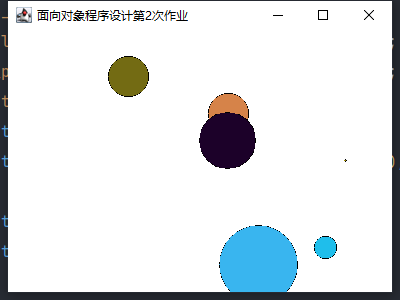
\includegraphics[width = 1\textwidth]{../pic/2/2.3.2.png}
		\caption{MyCircle 测试绘制结果}
	\end{subfigure}
\end{figure}

\begin{figure}[H]
	\centering
	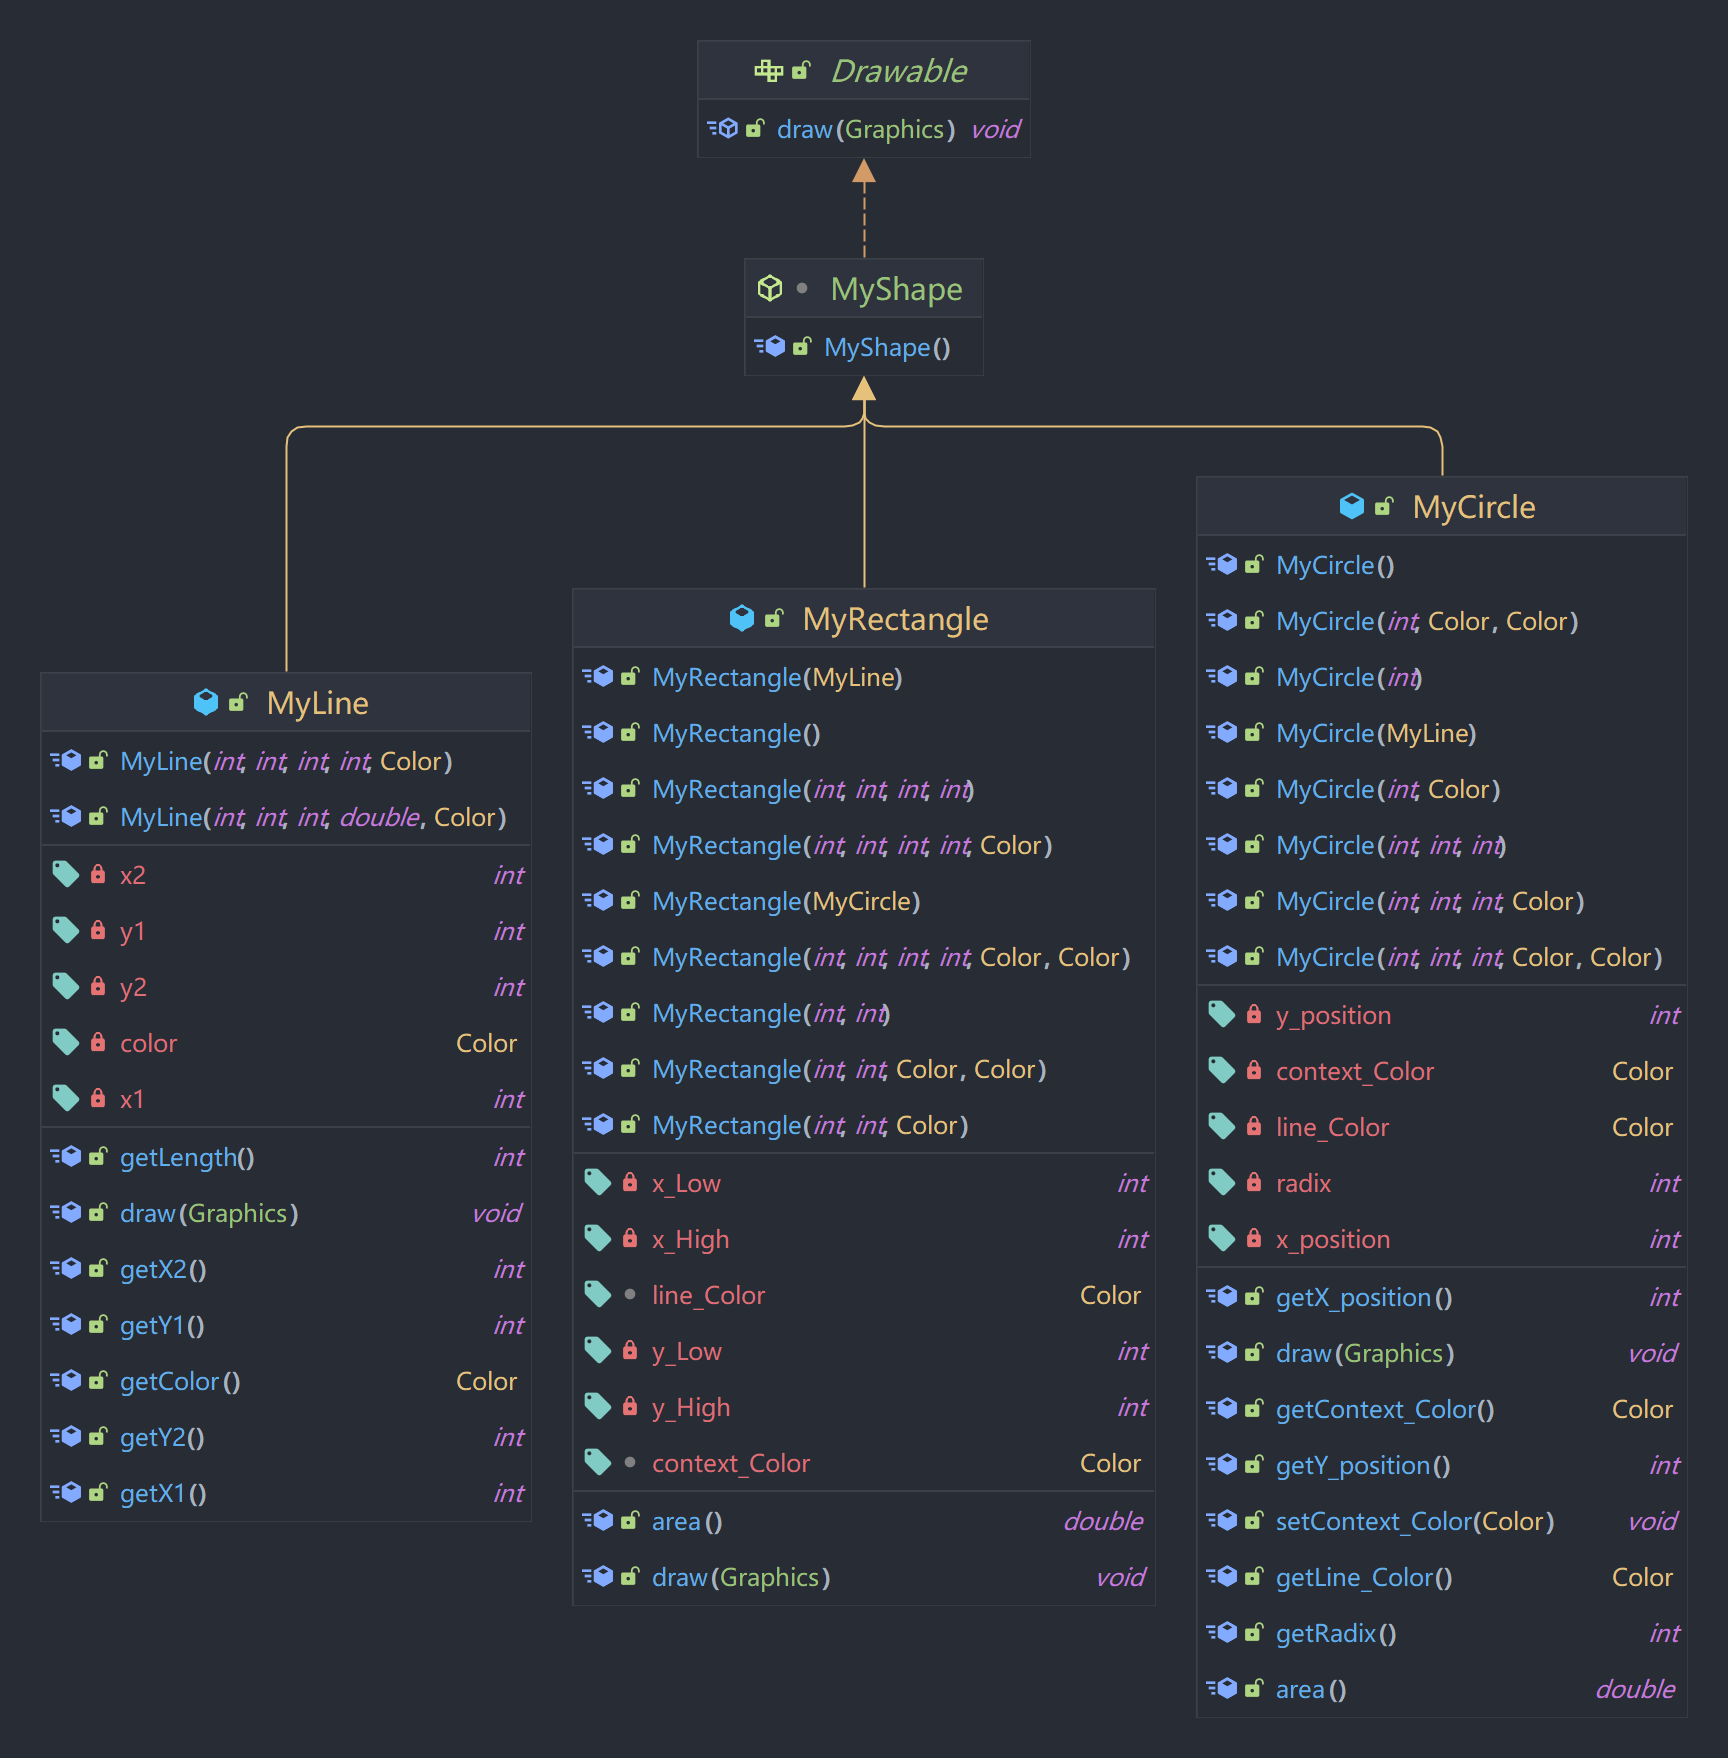
\includegraphics[width = 1\textwidth]{../pic/2/2.3.3.png}
	\caption{UML图}
\end{figure}

\section{2.4 主干代码说明}

\begin{lstlisting}[
	language = java,
	caption = {MyCircle.java L5-L86}
	]

public class MyCircle extends MyShape {
	private int x_position;
	private int y_position;
	private int radix;
	private Color context_Color;
	private Color line_Color;

	public MyCircle() {
		x_position = 0;
		y_position = 0;
		radix = 0;
		line_Color = Color.black;
		context_Color = Color.white;
	}

	public MyCircle(int r) {
		this();
		radix = r;
	}

	public  MyCircle(int r, Color cc) {
		this(r);
		context_Color = cc;
	}

	public  MyCircle(int r, Color cc, Color lc) {
		this(r, cc);
		line_Color = lc;
	}

	public MyCircle(int x, int y, int r) {
		this(r);
		x_position = x;
		y_position = y;
	}

	public MyCircle(int x, int y, int r, Color cc) {
		this(x, y, r);
		context_Color = cc;
	}

	public MyCircle(int x, int y, int r, Color cc, Color lc) {
		this(x, y, r, cc);
		line_Color = lc;
	}

	// Generate a circle taking line as diameter, just as an example, so no more Color-related method.
	public MyCircle(MyLine line){
		this(line.getX1()+ line.getX2() >>1, line.getY1()+ line.getY2()>>1,
				line.getLength()>>1, line.getColor());
	}

	public int getX_position() {
		return x_position;
	}

	public int getY_position() {
		return y_position;
	}

	public int getRadix() {
		return radix;
	}

	public void setContext_Color(Color cc){
		context_Color = cc;
	}

	public Color getContext_Color() {
		return context_Color;
	}

	public Color getLine_Color() {
		return line_Color;
	}

	public void draw(Graphics g) {
		g.setColor(line_Color);
		g.drawOval(x_position - radix, y_position - radix, 2*radix, 2*radix);
		g.setColor(context_Color);
		g.fillOval(x_position - radix, y_position - radix, 2*radix, 2*radix);
	}
\end{lstlisting}

\begin{lstlisting}[
	language = Java,
	caption = {MyRectangle.java L5-L71}
]
public class MyRectangle extends MyShape implements calcAreable {
	private int x_Low;
	private int y_Low;
	private int x_High;
	private int y_High;
	Color context_Color;
	Color line_Color;

	public MyRectangle() {
		x_Low = 0;
		y_Low = 0;
		x_High = 0;
		y_High = 0;
		line_Color = Color.black;
		context_Color = Color.white;
	}

	public MyRectangle(int x2, int y2) {
		this();
		x_High = x2;
		y_High = y2;
	}

	public MyRectangle(int x2, int y2, Color cc) {
		this(x2, y2);
		context_Color = cc;
	}

	public MyRectangle(int x2, int y2, Color cc, Color lc) {
		this(x2, y2, cc);
		line_Color = lc;
	}

	public MyRectangle(int x1, int y1, int x2, int y2) {
		this(x2, y2);
		x_Low = x1;
		y_Low = y1;
	}

	public MyRectangle(int x1, int y1, int x2, int y2, Color cc) {
		this(x1, y1, x2, y2);
		context_Color = cc;
	}

	public MyRectangle(int x1, int y1, int x2, int y2, Color cc, Color lc) {
		this(x1, y1, x2, y2, cc);
		line_Color = lc;
	}

	// Generate a rectangle taking line as diagonal just as an example, so no more Color-related method.
	public MyRectangle(MyLine line) {
		this(Math.min(line.getX1(), line.getX2()), Math.min(line.getY1(), line.getY2()), Math.max(line.getX1(), line.getX2()), Math.max(line.getY1(), line.getY2()), line.getColor());
	}

	public MyRectangle(MyCircle circle) {
		this(circle.getX_position() - circle.getRadix(), circle.getY_position() - circle.getRadix(), circle.getX_position() + circle.getRadix(), circle.getY_position() + circle.getRadix(), circle.getContext_Color(), circle.getLine_Color());
	}

	public void draw(Graphics g) {
		g.setColor(line_Color);
		g.drawRect(x_Low, y_Low, x_High - x_Low, y_High - y_Low);
		g.setColor(context_Color);
		g.fillRect(x_Low, y_Low, x_High - x_Low, y_High - y_Low);
	}
\end{lstlisting}

\lstinputlisting[language = Java, caption = {MyShape.java}]{../../../ProblemSet/src/hw2/p2/MyShape.java}

\lstinputlisting[language = Java, caption = {Drawable.java}]{../../../ProblemSet/src/hw2/p2/Drawable.java}

\lstinputlisting[language = Java, caption = {DrawPanel.java}]{../../../ProblemSet/src/hw2/p2/DrawPanel.java}

\section{2.6 总结和收获}

本题更像作为作业1和作业3的衔接,第一个任务以更大的可扩展性让我练习了构造函数的设计方法,这让我对利用 this() 在构造函数间相互调用更加得心应手。
而通过查阅官方文档了解 Graphics 的类方法并上手使用则锻炼了我阅读文档的能力。

第二个任务虽然可以只单纯地抽象一层,即设计一个父类囊括所有图形,但看过作业三后就知道这里如果再抽象一层接口出来会更好,
即 DrawPanel 不用局限于 MyShape 类。但这样设计需要考虑一个新的问题: MyShape 类是否还有存在的必要?经过思考后我的解决方案是保留
 MyShape 类,因为之后可能会添加其他的图形类的共性。这种抽象几层和类存在必要性的斟酌对我对面向对象设计的理解很有帮助。

% 1、题目
% 2、数据设计
% 3、算法设计
% 4、主干代码说明
% 5、运行结果展示
% 6、总结和收获